\chapter{System Design}\label{Lit:sysDesign}
%%%%%%%%%%%%%%%%%%%%
\section{Charging circuit overview}
The charging circuit structure can be seen in figure \ref{fig:A2block} as the green highlighted blocks. The 12V supply and the solar panel will connect directly to the linear regulator. The linear regulator is the part of the system that will be tuned to achieve the adequate current limiting, voltage and thermal specifications. The charging circuit will then be intercepted by the high side switch so that the charging can be controlled by a logic high or low to the switch. 

\begin{figure}[!htb]
\centering
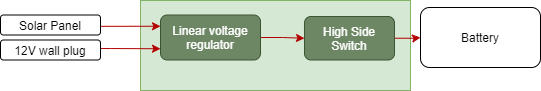
\includegraphics[scale=0.5]{./Figures/A2}
\caption{Charging System Block Diagram}
\label{fig:A2block}
\end{figure}

%%%%%%%%%%%%%%%%%%%%%%%
\section{Under Voltage and Over Current circuit overview}
The circuit structure can be seen in figure \ref{fig:A3block} as the yellow highlighted blocks. The goal of this circuit is to disconnect the battery from the load when the voltage is below a certain voltage and then to reconnect the battery when the voltage is above a certain voltage. The circuit will also protect the battery from abnormally high charging currents with a fuse. The Schmidt trigger block manages the logic of whether the switch should be on or off. This decision is then conveyed to the high side switch which then implements the connection or disconnection of the battery from the load. In order for the Schmidt trigger to work it requires 5V which will be supplied through a regulator from the battery.

\begin{figure}[!htb]
\centering
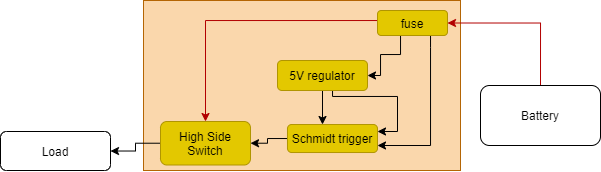
\includegraphics[scale=0.5]{./Figures/A3}
\caption{Under Voltage System Block Diagram}
\label{fig:A3block}
\end{figure}

%%%%%%%%%%%%%%%%%%%%%%%%%%%%%%%
\section{Current sense circuit overview}
The current sense circuit structure can be seen in figure \ref{fig:finalblock} as the purple highlighted blocks. The current sense circuit connects the two previous system block diagrams to make up the final block diagram.  The current sense circuitry was added at its position after the load so that the current it will measure is the current discharging from the battery or charging into the battery. In order to operate the current sense amplifier will require a 5V from the 5V regulator.  The current sense amplifier will be used to produce voltage between 0V and 5V that will correspond proportionally to the current in a designed range of 3V. The current sense amplifier will amplify very small voltages across the current sense resistor. The load can also be connected and disconnected with the help of the designed low side switch. The output of the current sense amplifier will be prone to noise from the 12V wall plug as well as the 5V regulator. In order to fix this a output filter will be required at the output of the current sense amplifier. The directions of the arrows in the block diagrams show the direction that current flow will be enforced. This means schottky diodes will be used at the solar panel the 12V wall plug as well as the output of the charging circuit. 
%%%%%%%%%%%%%%%%%%%%%%%%%%%%%%%%



\begin{figure}[!htb]
\centering
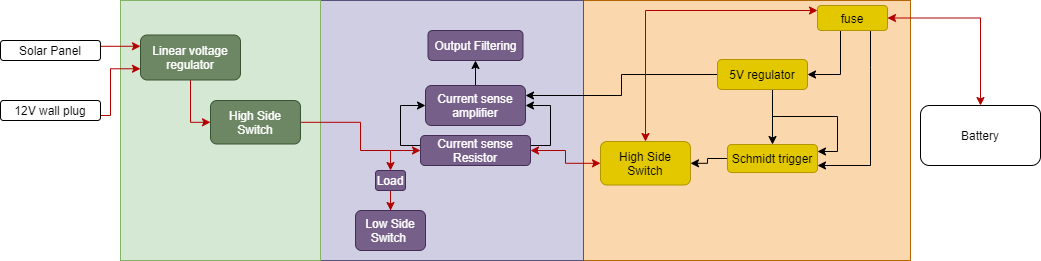
\includegraphics[scale=0.45]{./Figures/A5}
\caption{Complete System Block Diagram}
\label{fig:finalblock}
\end{figure}


\section{Battery and Supply voltage measurement}




